\epigraph{\emph{
  ``If I have seen further it is by standing on the shoulders of giants.''
}}{ Isaac Newton }

The goal of this section is to give some intuition and the necessary theoretical background for the following chapters. The areas where clustering problems arise are huge. It provides solutions to problems like market segmentation, classification, document organization or indexing.\\
Firstly we will have a look at the definition of clustering and summarization. How they are related and the variety of possibilities this imposes.
Secondly the vector space model (VSM) is introduced. It contains all information about how to represent documents in a vectorized form. Of special interest are enhanced models which reduce the dimensionality of documents by singular value decomposition (SVD).
Thirdly traditional clustering algorithms from the hierarchical (Ward, Birch) and partitional (K-Means, Mean-Shift) will be presented.
Closely related are the generative models. These methods can be used as a kind of clustering algorithm and are highly useful in several steps of traditional clustering. They can be used as dimensionality reduction techniques as well.
Lastly some quality measures of clusters based on internal measures (without ground truth labels) and external measures (with explicit labelling of the ground truth) are explained.


\section{Clustering and Summarization}
  
  \textbf{Clustering} as defined by \cite{ClusterAlgoSurveyIBM} is finding groups of similar objects in the data with a defined similarity function between objects. The granularity of the features can vary:

  \begin{itemize}
    \item \emph{Sentence based} - A document d is split into sentences so clustering reveals the most coherent groups of sentences that are closely related.
    \item \emph{Collection of documents} - A collection of documents d (corpora) is grouped to get groups of documents that are closely related
    \item \emph{Stream of documents} - The same as clustering copora with the constraint that over time the size of documents grow.
  \end{itemize}

  Document clustering on large corpora can be seen as a summarization of the underlying concepts. The representation of documents as feature vectors is described with the vector space model in the next section.\\
  \textbf{Automatic text summarization} on the other hand, is the process of reducing textual content to the most important concepts in a readable, formatted form to the user \cite{SumEvaluation2001}.\\
  This results in a few possibilities where clustering works great as a preprocessing step for summarization.
  
  \begin{description}
    \item[First] Clustering groups that have a \emph{higher density of information} resulting in a grouped input for summarizers.
    \item[Second] Grouping the \emph{latent topics} accross and within documents to create a meta concept of closely related documents
    \item[Third] Classify documents into \emph{categories} in a semi supervised way to construct hierarchies of relationships
    \item[Fourth] Finding \emph{outliers} that will not highly contribute to the summarization
  \end{description}

  Aside clustering itself can be seen as a summarization as well. Clustering can lead to well formed topical browsers where users can interact with a graphical user interface to browse topics in a more coherent and semantic way see \cite{Carrot2Search2003}.

  \paragraph{Supervision}

    As opposed to unsupervised learning strategies such as clustering, supervised learning classifies some input based on a provided ground truth. That is for an input \emph{x} there are labels \emph{y} that describe the class they are in. Supervision can be done by explicitly classifying the documents before the clustering. The input is then split into \emph{n} classes. Then each class can be individually clustered. Often however this is no option. We need to manually label all documents. This can be time consuming and error prone. Often several labellers are needed to crossvalidate human bias.
    With this in mind there are two options on how to label unseen or new data:

      \begin{itemize}
        \item Use a supervised classification algorithm to automatically label unlabelled data. A prerequisite is to have a labelled training set and to have a lot of data. To name a few candidates: \emph{Multinominal/Gaussian) Naive Bayes (NB)}, \emph{Multivariate Logistic/Linear Regression}, \emph{Neural Networks (ANN)}, \emph{Support Vector Machines (SVM)} or \emph{Random Forests (RF)}.
        \item Use an unsupervised clustering algorithm to automatically label unlabelled data. This can be done by first forming clusters and then merging the nearest clusters until k distinct categories remain. Usually the merging criterion can be controlled by some threshold and high variance documents are sorted out into an outlier cluster.
      \end{itemize}

    Usually by clustering we mean automatic detection of the grund truths. Often this is to shallow and does not lead to labels with a high confidence. In the domain of document clustering all information that provide some context are critical and should be used.

\newpage{}
\section{Vector Space Model (VSM)}
  
  \paragraph{}
    The vector space model is directly derived from the vector space which is studied in linear algebra. If we talk about vector space we often refer to the euclidean vector space where the dimensions are typically not higher than 3 dimensions. All dimensions higher than 3 are hard to display and to imagine. However this is does not mean that the rules do not hold true for higher dimensions.

  \begin{figure}[h!]
    \centering
      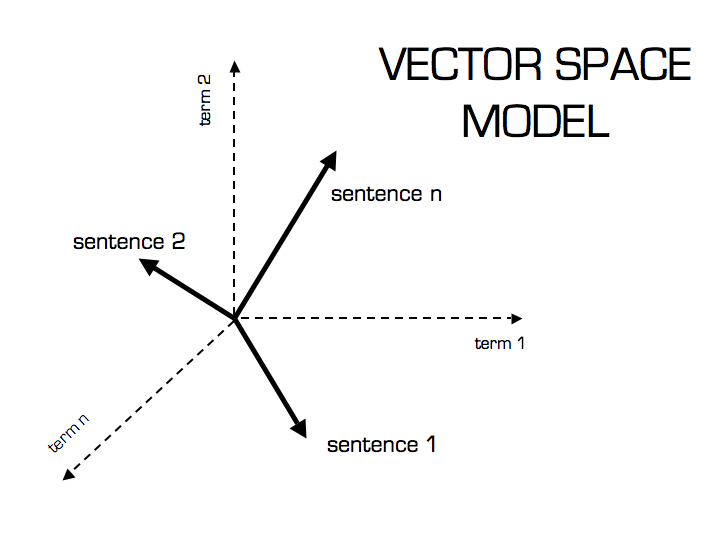
\includegraphics[width=0.7\textwidth]{vsm.png}
      \caption{"Fig. 1 - Vector space model"}
      \label{vsm_pic}
  \end{figure}

  \paragraph{}
    The vector space model in the text domain has the meaning that each word is a component of a document. If a document has 100 distinct words, the resulting document vector is in 100th dimensional space. If a second document has 50 distinct words, independant of the first document, vectors are now in 150th dimensional space but with the non existant words set to 0. In linear algebra we can interpret two documents as two vectors forming a subspace in an \emph{m x n} matrix where m is the document size and \emph{n} all the features from all documents. It is typical that we generally have a lower \emph{m} and a much higher \emph{n} resulting in highly sparse vectors with a lot of zeros, typically 99\%. This also results in feature explosion where no document is close to one another because the dimensions are too high.\\
    \emph{Simple example: Take 500 documents with 500 words and each document has a few words in common with another one, you easily get 200.000 features. Even documents with a lot of common or shared words will not be very close then.}

  \subsection{Notation}
  \subsection{Bag of words}
  \subsection{Similarity and Distances}
  \subsection{Dimensionality and Hashing}

  \subsection{Enhancing the Vector Space Model}
    \subsubsection{Singular Value Decomposition (SVD)}
    \subsubsection{Latent Semantic Analysis (LSA)}
    \subsubsection{Principal Component Analysis (PCA)}

\section{Clustering algorithms}

  \subsection{Objective goal}
    EM, Cost functions, general clustering scheme

  \subsection{Hierarchical / Agglomerative clustering}
    \paragraph{Ward, Complete and Average Linkage}
    \paragraph{Birch}

  \subsection{Partitional clustering}
    \paragraph{K-Means}
    \paragraph{Mean-Shift}

    \subsection{Others}
      \begin{enumerate}
        \item \emph{Spectral} - x
        \item \emph{Density} - x
        \item \emph{Grid} - x
      \end{enumerate}


\section{Generative Models}    
  
  \subsection{Topic modelling}
    \paragraph{Bayes Theorem}
    \paragraph{Multinominal Distributions}
    \paragraph{Dirichlet Distributions}
      Chinese Restaurant Process

  \subsection{Methods}
    \subsubsection{Latent Dirichlet Allocation (LDA)}
    \subsubsection{Non Negative Matrix Factorization (NMF)}


\section{Clustering quality measures}

  \subsection{Internal measures}
    Without labels of the ground truth

    \begin{enumerate}
      \item \emph{Silhouette coefficient} - x
      \item \emph{Davies–Bouldin index} - x
      \item \emph{Dunn index} - x
    \end{enumerate}

  \subsection{External measures}
    With labels of the ground truth

    \begin{enumerate}
      \item \emph{F-Measure} - x
      \item \emph{Jaccard index} - x
    \end{enumerate}

